\begin{figure}[t]
\centering
\small
\begin{tabular}{@{}cc@{}}
\multicolumn{2}{c}{\textbf{Inputs supplied to the model}}\\[3pt]
Crease pattern & Target folded state\\
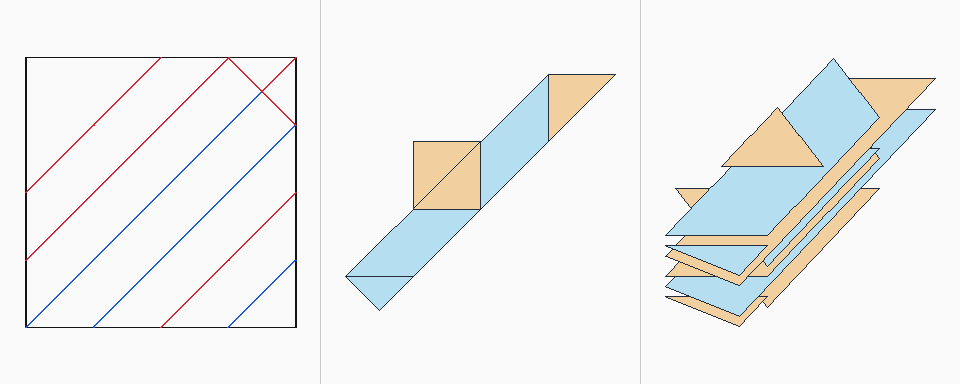
\includegraphics[width=2.5cm,trim=0 0 640bp 0,clip]{figures/dataset/sample-1.png}&
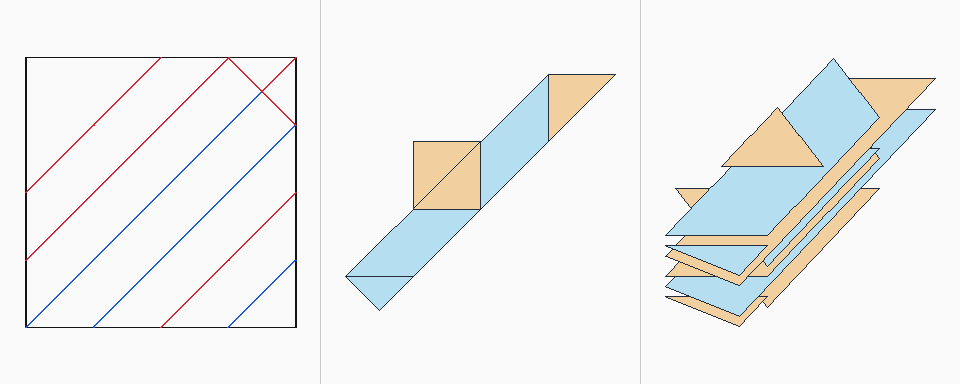
\includegraphics[width=2.5cm,trim=320bp 0 320bp 0,clip]{figures/dataset/sample-1.png}
\end{tabular}
\par\medskip
\textbf{Required output: an executable folding sequence}\par\smallskip
\resizebox{.96\linewidth}{!}{%
\begin{tabular}{@{}ccccc@{}}
Unfolded & Fold 1 & Fold 2 & Fold 3 & Fold 4\\[2pt]
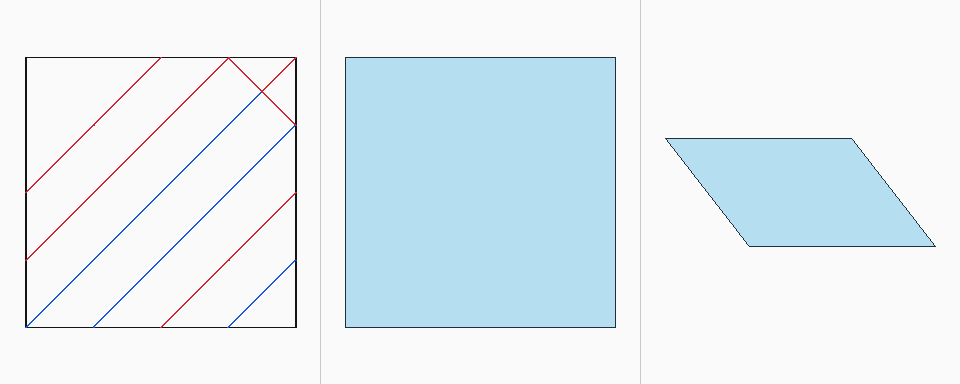
\includegraphics[width=2cm,trim=320bp 0 320bp 0,clip]{figures/dataset/sample-1-state-0.png}&
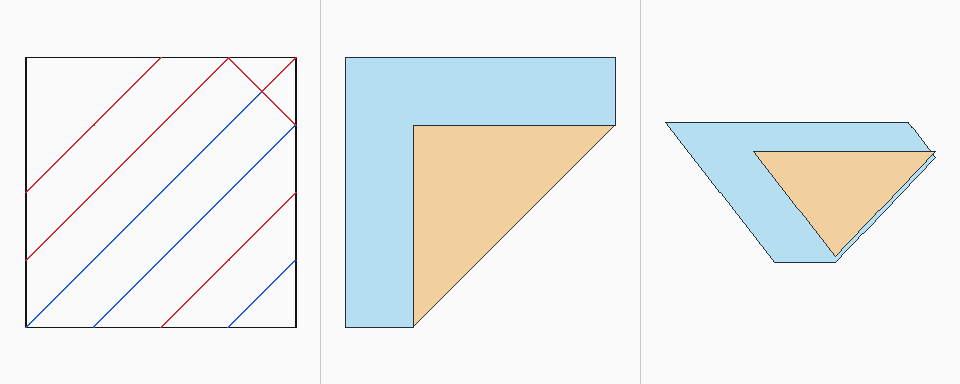
\includegraphics[width=2cm,trim=320bp 0 320bp 0,clip]{figures/dataset/sample-1-state-1.png}&
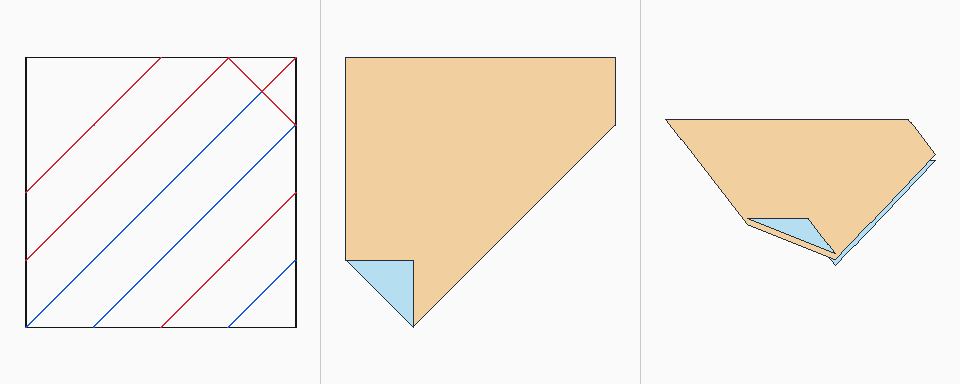
\includegraphics[width=2cm,trim=320bp 0 320bp 0,clip]{figures/dataset/sample-1-state-2.png}&
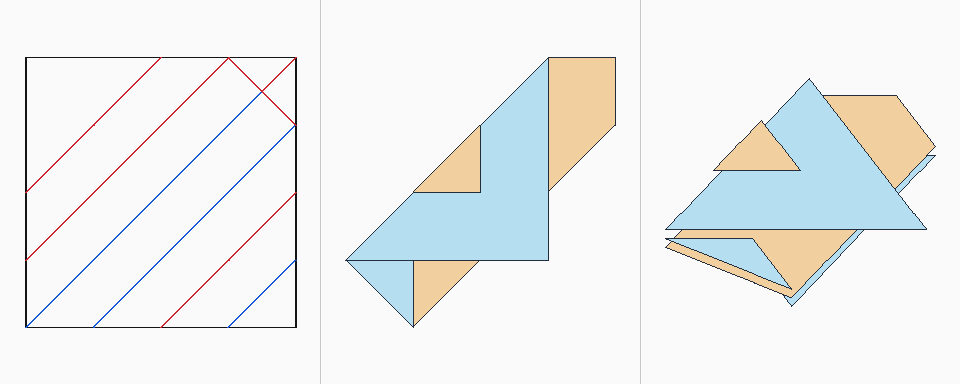
\includegraphics[width=2cm,trim=320bp 0 320bp 0,clip]{figures/dataset/sample-1-state-3.png}&
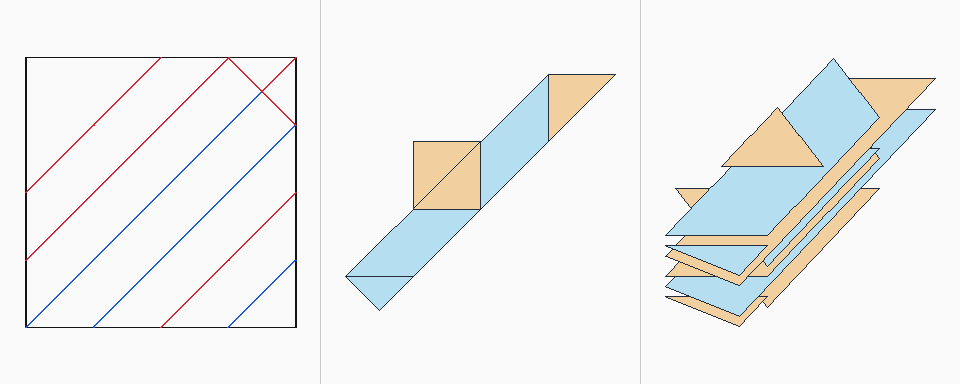
\includegraphics[width=2cm,trim=320bp 0 320bp 0,clip]{figures/dataset/sample-1-state-4.png}\\
& $\longrightarrow$ & $\longrightarrow$ & $\longrightarrow$ & $\longrightarrow$
\end{tabular}}
\caption{CP2Seq task illustrated by all-layers/easy-0001. The model receives the crease pattern
and target state and must produce a valid sequence from the unfolded sheet. The lower row shows
the recorded reference sequence, which is withheld during evaluation.}
\label{fig:sample}
\end{figure}
